\chapter{Zagadnienia powiązane z wizyjnym śledzeniem obiektów}
\label{cha:Zagadnienia_powiazane_z_wizyjnym_sledzeniem_obiektow}

\section{Ekstrakcja i deskrypcja cech obrazu}
\label{sec:Ekstrakcja_i_deskrypcja_cech_obrazu}
Pojęcie \textbf{cechy obrazu} (ang. \textit{image feature}) jest z natury nieprecyzyjne i ogólnie może oznaczać dowolną informację związaną z obrazem, która jest przydatna w ramach wykonywania określonego algorytmu. Funkcjonuje ono w literaturze również w nieco konkretniejszym ujęciu i według monografii \cite{Szeliski2011} obiekty określane cechami obrazu należą do jednej z trzech podstawowych kategorii:

\begin{enumerate}
	\item Punkty charakterystyczne (ang. \textit{keypoint features}, \textit{interest points} lub \textit{corners}) i regiony charakterystyczne (ang. \textit{blobs})
	\item Kontury obiektów na obrazie (ang. \textit{edges})
	\item Proste oraz krzywe występujące na obrazie
\end{enumerate}

Porównanie przykładowych cech obrazów należących do poszczególnych kategorii przedstawione zostało na rysunku \ref{fig:Przyklady_cech}. Ekstrakcja i deskrypcja cech jest jedną z podstawowych metod analizy obrazów i znajduje zastosowanie m.in. w algorytmach rozpoznawania obiektów, śledzenia obiektów, mozaikowania czy dopasowywania obrazów w stereoskopii. Celem wykonania takiej operacji jest wydobycie z dużej ilości informacji zawartej na obrazie jej istotnej części.

\begin{figure}[!htb]
	\begin{center}
		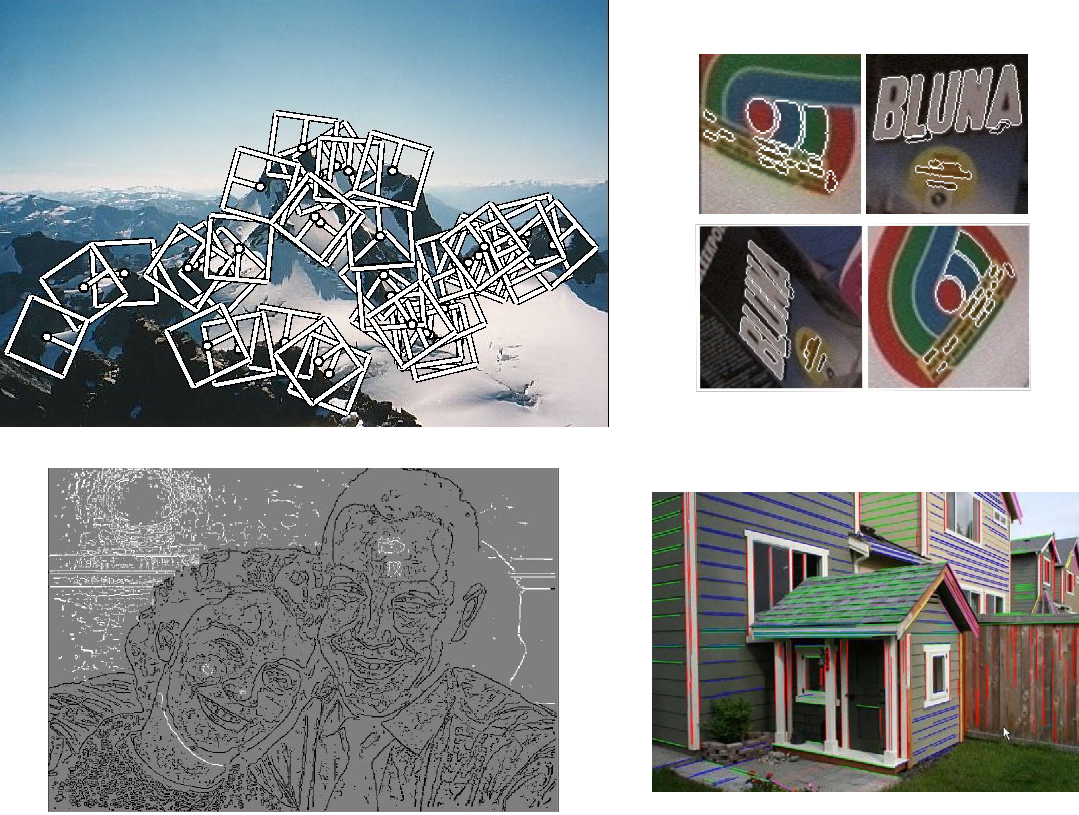
\includegraphics[width=12cm]{images/object_features.png}
	\end{center}	
	\longcaptionsource{Przykłady cech występujących na obrazach}{Od lewego górnego rogu: Punkty charakterystyczne (tutaj z wizualizacją ich przykładowych deskryptorów), regiony charakterystyczne, kontury obiektów, linie proste występujące na obrazie}{\cite{Szeliski2011}}
\label{fig:Przyklady_cech}
\end{figure}

\subsection{Punkty charakterystyczne}
\label{subsec:Punkty_charakterystyczne}
\textbf{Punkt charakterystyczny} można rozumieć jako punkt na obrazie wyróżniający się spośród otoczenia, np. narożnik występujący w konturze obiektu widocznego na obrazie. Analogicznie, \textbf{region zainteresowania} posiada cechę charakterystyczną odróżniającą go od tła, np. ma jednolity kolor. W obu przypadkach stwierdzenie ,,charakterystyczności'' odbywa się poprzez porównanie z otoczeniem. Porównanie to polega zwykle (w dużym uproszczeniu) na znalezieniu maksimów lokalnych pewnej funkcji oceniającej ,,charakterystyczność'' dla każdego punktu obrazu oraz jego lokalnego otoczenia. Po wykryciu zbioru cech wykonuje się ich \textbf{deskrypcję} (ang. \textit{feature description}), polegającą na wyznaczeniu ich formalnego opisu (zwykle w postaci wektora liczb) cechującego się zwięzłością, powtarzalnością oraz inwariantnością \cite{Szeliski2011}, tzn. odpornością na przekształcenia afiniczne, zmiany oświetlenia, szum, etc. Odbywa się to w oparciu o piksele otoczenia punktu charakterystycznego lub piksele samego regionu charakterystycznego. Granica rozróżniająca punkt charakterystyczny i region charakterystyczny jest więc bardzo niewyraźna, tym niemniej występuje w literaturze. Analizę z wykorzystaniem cech tego typu kończy ich \textbf{dopasowanie} (ang. \textit{feature matching}) lub \textbf{śledzenie} (ang. \textit{feature tracking}), np. pomiędzy dwoma kolejnymi klatkami sekwencji video lub obrazami jednej sceny zarejestrowanymi przy użyciu dwóch kamer. Model w postaci zbioru lokalnych cech, którymi są punkty charakterystyczne, nie wymaga żadnych założeń dotyczących wyglądu czy charakterystyki reprezentowanego obiektu jak całości, jak to ma miejsce np. w przypadku reprezentacji konturem. Czyni to punkty charakterystyczne odpowiednią metodą opisu obiektu w przypadku występowania zmian oświetlenia, przysłonięć i innych zakłóceń występujących powszechnie w rzeczywistych, użytkowych sekwencjach video \cite{Treiber2010}.

Ze względu na dużą użyteczność, algorytmy ekstrakcji i deskrypcji puntów charakterystycznych stanowiły w ostatniej dekadzie przedmiot intensywnych badań \cite{Treiber2010}. W literaturze zaproponowano wiele różnych podejść do tego zagadnienia, jednak jako najważniejszy przykład, dobrze obrazujący poszczególne etapy jego realizacji wymienia się algorytm \textit{SIFT} (\textit{Scale-Invariant Feature Transform}) \cite{Treiber2010} \cite{Szeliski2011}. Wykryte przy jego pomocy punkty charakterystyczne cechują się inwariantnością na zmiany skali i rotacji obrazu, a także częściowo na zmiany oświetlenia oraz zmiany widoku wynikającej z przesunięcia kamery rejestrującej scenę. Dodatkowo wykazują one dużą specyficzność (tzn. cechy odpowiadające poszczególnym fragmentom obrazu znacznie się między sobą różnią), zaś sam algorytm jest efektywny obliczeniowo \cite{Lowe2004}. Opis działania metody \textit{SIFT} zostanie poniżej przytoczony w całości.

Pierwszym krokiem algorytmu jest wyznaczenie reprezentacji obrazu w \textbf{przestrzeni skali} (ang. \textit{scale space}), w której informacja przechowywana w jego pikselach zależy nie tylko od ich współrzędnych $x$, $y$ ale również od skali $s$. Pozwala to na wykrycie punktów charakterystycznych, które pozostają stabilne przy zmianie tej skali \cite{Treiber2010}. Reprezentacja obrazu w przestrzeni skali wyznaczana jest zgodnie ze wzorem:
\begin{equation}
\label{equ:Obraz_w_przestrzeni_skali}
	L(x, y, \sigma) = G(x, y, \sigma) \ast I(x, y)
\end{equation}

\begin{equation}
\label{equ:Filtr_Gaussa}
	G(x, y, \sigma) = \dfrac{1}{\sqrt{2 \pi} \sigma ^ 2 } e^{-(x^2+y^2) / 2 \sigma^2}
\end{equation}

\noindent
gdzie:

\begin{conditions}
	x,y	& współrzędne piksela na obrazie \\
	I(x,y) & wartość piksela o współrzędnych $(x,y)$ na obrazie $I$ \\
	L(x,y,\sigma) & reprezentacja obrazu w przestrzeni skali w punkcie $(x,y)$ \\
	\sigma & rozmiar maski dla filtru Gaussa, definiujący skalę $s$ \\
	G(x,y,\sigma) & wartość maski Gaussa o rozmiarze $\sigma$ dla piksela o współrzędnych $(x,y)$\\
	\ast & operator konwolucji \\
\end{conditions}

Punkty charakterystyczne znajdują się w lokalizacjach wystąpień lokalnych minimów i maksimów reprezentacji obrazu w przestrzeni skali $L$. W celu ich wyznaczenia obliczana jest różnica obrazów w sąsiednich skalach $D(x, y, \sigma)$ \cite{Lowe2004}:
\begin{equation}
\label{equ:Roznica_obrazow}
	D(x, y, \sigma) = (G(x, y, k \sigma) - G(x, y, \sigma)) \ast I(x, y) = L(x, y, k \sigma) - L(x, y, \sigma)
\end{equation}

\noindent
gdzie:

\begin{conditions}
	k & stały współczynnik (zwykle $k \in [1,1 ; 1,4]$) \\
	D(x, y, \sigma) & Różnica filtrów Gaussa, w skrócie \textit{DoG} (z ang. \textit{Difference of Gaussian})   
\end{conditions}

Przeszukiwanie przestrzeni skali odbywa się poprzez wielokrotne wyznaczenie $D(x, y, \sigma)$, któremu towarzyszy zwiększanie $\sigma$ o stałą wartość. Lokalne ekstrema wyznaczane są poprzez porównywanie wartości $D(x, y, \sigma)$ dla współrzędnych $(x, y, \sigma)$ z punktami sąsiadującymi z punktem $(x, y)$ w skali określonej przez $\sigma$ oraz dwoma regionami o wymiarach $3 \times 3$, współśrodkowymi z $(x, y)$, o sąsiednich skalach \cite{Lowe2004}.

W ten sposób otrzymywany jest zbiór punktów charakterystycznych o określonych współrzędnych $(x, y)$ oraz skali $\sigma$. Pozycja określona tymi współrzędnymi jest jednak niedokładna - punkt charakterystyczny
może znajdować się pomiędzy pikselami (które stanowią próbki pomiarowe), dodatkowo jeden piksel w niżej skali odpowiada wielu pikselom w wyższej. Położenie ekstremów $\hat{\vec{x}}$ jest wyznaczane na podstawie interpolacji funkcją kwadratową wyznaczanej poprzez rozwinięcie w szereg Taylora funkcji $G(x, y, \sigma)$ \cite{Lowe2004}:

\begin{equation}
\label{equ:Ekstrema_interpolacja}
	\hat{\vec{x}} = - \frac{\partial^2 D^-1}{\partial \hat{\vec{x}}^2} \frac{\partial D}{\partial \hat{\vec{x}}}
\end{equation}

\noindent
gdzie:

\begin{conditions}
	\hat{\vec{x}} & wektor współrzędnych w przestrzeni skali
\end{conditions}

Dodatkowo zbiór ekstremów jest filtrowany - odrzucane są niestabilne punkty charakterystyczne o niskim kontraście \cite{Lowe2004}.

\begin{equation}
\label{equ:Filtrowanie}
	D(\hat{\vec{x}}) = D + \frac{1}{2} \frac{\partial D^T}{\partial \vec{\vec{x}}} \hat{\vec{x}}
\end{equation}

Ekstrema o wartości bezwzględnej $\abs{D(\hat{x})}$, obliczonej na podstawie równania \ref{equ:Filtrowanie}, mniejszej od wartości progowej $0.03$ są usuwane ze zbioru punktów charakterystycznych \cite{Lowe2004}.

Operacja \textit{DoG} silnie reaguje na krawędzie obecne na obrazie, co jest zjawiskiem niepożądanym, ponieważ ma charakter kierunkowy i skutkuje zdefiniowaniem niestabilnych punktów charakterystycznych
\cite{Lowe2004}. W celu ich eliminacji wprowadza się drugi etap filtracji, polegający na wyznaczeniu hesjanu $H$ (równanie \ref{equ:Hesjan}) i porównaniu jego śladu i wyznacznika z wartością progową(równanie \ref{equ:Hesjan_prog}).

\begin{equation}
\label{equ:Hesjan}
	\matr{H} = \begin{bmatrix}
		D_{xx} & D_{xy} \\
		D_{yx} & D_{yy} \\
	\end{bmatrix}
\end{equation}

\begin{equation}
\label{equ:Hesjan_prog}
	\frac{\Tr{\matr{H}}^2}{\Det{\matr{H}}} < \frac{(r + 1)^2}{r}
\end{equation}

\noindent
gdzie:
\begin{conditions}
	r & wartość progowa \\
\end{conditions}

Osiągnięcie inwariantności na obrót obrazu uzyskuje się poprzez przypisanie punktom charakterystycznym orientacji \cite{Lowe2004}. Na podstawie skali $\sigma$ punktu wyznacza się w jego środku maskę Gaussa o wariancji równej $1,5$ jego skali, w obrębie której wyznacza się moduł (równanie \ref{equ:Gradient_modul}) oraz orientację (równanie \ref{equ:Gradient_orientacja}) gradientu dla każdego piksela $(x, y)$.

\begin{equation}
\label{equ:Gradient_modul}
	m(x,y) = \sqrt{(I_s(x + 1, y) - I_s(x - 1, y))^2 + (I_s(x, y + 1) - I_s(x, y - 1))^2}
\end{equation}

\begin{equation}
\label{equ:Gradient_orientacja}
	\theta(x,y) = \arctan(\frac{I_s(x, y + 1) - I_s(x, y - 1)}{I_s(x + 1, y) - I_s(x - 1, y)})
\end{equation}

Obliczone orientacje są następnie kumulowane w histogramie z wagami określonymi poprzez odpowiadające im moduły oraz wartości okna Gaussa. Histogram składa się z $36$ przedziałów odpowiadających $360 \deg$ orientacji. Przedziały o największej liczebności odpowiadają dominującym orientacjom \cite{Lowe2004}, przy czym punktowi przypisywana jest orientacja odpowiadająca najliczniejszemu przedziałowi oraz wszystkie inne orientacje, dla których liczebności wynoszą przynajmniej $80 \%$ maksymalnej (punkt może mieć wiele orientacji jednocześnie).

\begin{figure}[!htb]
	\begin{center}
		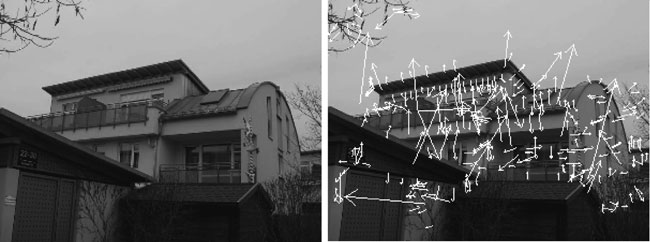
\includegraphics[width=12cm]{images/sift_extraction_description_example.png}
	\end{center}	
	\longcaptionsource{Przykład ekstrakcji i deskrypcji punktów charakterystycznych metodą \textit{SIFT}}{Punkty charakterystyczne zlokalizowane są w początkach białych strzałek, wizualizujących ich dominujące orientacje (kierunek) oraz skale (długość). Na przykładowym obrazie wykryto 289 punktów charakterystycznych.}{\cite{Treiber2010}}
\label{fig:SIFT_przyklad}
\end{figure}

Na podstawie lokalnych orientacji wyznaczany jest również deskryptor punktu charakterystycznego. Na region o wymiarach $16 \times 16$ pikseli o środku w punkcie charakterystycznym nakładana jest maska Gaussa o wariancji równej połowie jego wielkości. Następnie region ten jest dzielony na tablicę $4 \times 4$ podregionów, w obrębie których następuje akumulacja orientacji w histogramach o $8$ przedziałach (analogicznie jak w wyznaczaniu orientacji samego punktu, z wagami odpowiadającymi modułowi oraz wartości okna Gaussa) \cite{Lowe2004}. W ten sposób powstaje wektor zawierający $4 \times 4 \times 8 = 128$ elementów, opisujących punkt charakterystyczny. Końcowym etapem algorytmu jest wykonanie normalizacji, progowania ograniczającego wartość elementów do $0.2$ (próg wyznaczony eksperymentalnie) oraz renormalizacji. W ten sposób uzyskiwana jest inwariantność na zmiany iluminacji \cite{Lowe2004}. Deskryptory pozwalają na wykonanie dopasowania pomiędzy punktami charakterystycznymi (np. wykrytymi na dwóch różnych ujęciach, przedstawiających ten sam obiekt), np. przy pomocy algorytmu k-najbliższych sąsiadów (ang. \textit{k nearest neighbours}) z zastosowaniem metryki euklidesowej. Przykładowy wynik ekstrakcji i deskrypcji punktów charakterystycznych z wykorzystaniem algorytmu \textit{SIFT} przedstawiono na rysunku \ref{fig:SIFT_przyklad}.

\subsection{Krawędzie}
\label{subsec:Krawedzie}
Pomimo swoich zalet, punkty charakterystyczne nie zawsze stanowią optymalny sposób reprezentacji cech obiektu. Istnieje liczna grupa zagadnień, w których istotna jest informacja o obiekcie jako o całości, w szczególności o jego właściwościach geometrycznych. Przykładowo, są one kluczowe w zadaniu automatycznego rozpoznawania znaków drogowych lub wykrywania produktów na przenośniku taśmowym w oparciu o szablony zdefiniowane w postaci ich modeli CAD \cite{Treiber2010}. W takich przypadkach analizę obrazu przeprowadza się w oparciu o wykryte na nim \textbf{krawędzie}.

Krawędzie można zdefiniować jako granice pomiędzy regionami obrazu o różnym kolorze, intensywności bądź teksturze \cite{Szeliski2011}. Wykrywanie tych granic jest jednak zadaniem trudnym i stanowi osobną, złożoną dziedzinę cyfrowego przetwarzania obrazów noszącą nazwę segmentacji \cite{Szeliski2011}. Alternatywnie, na potrzeby zadania ekstrakcji cech, krawędzie można zdefiniować w ujęciu ,,lokalnym'' - jako wystąpienia nagłych zmian intensywności pikseli, czyli formalnie jako punkty, w których modułu lokalnego gradientu funkcji intensywności (równanie \ref{equ:Gradient_definicja}) przyjmuje duże wartości \cite{Szeliski2011}.

\begin{equation}
\label{equ:Gradient_definicja}
	\vec{J}(\vec{x}) =  \nabla I (\vec{x}) = (\frac{\partial I}{\partial x}, \frac{\partial I}{\partial y})(\vec{x})
\end{equation}

\noindent
gdzie:

\begin{conditions}
	\vec{J}(\vec{x}) & wartość gradientu funkcji intensywności dla współrzędnych $\vec{x}$ \\
	\vec{x} & wektor współrzędnych piksela $(x, y)$ \\
\end{conditions}

W praktyce obliczanie gradientu obrazu polega na wykonaniu jego splotu z odpowiednimi maskami, mającymi charakter kierunkowy. W wyniku takiej operacji otrzymuje się przybliżone pochodne kierunkowe obrazu, na podstawie których można następnie wyznaczyć moduł i orientację gradientu. Operacja wyznaczenia pochodnej obrazu wzmacnia wpływ składowych o wysokiej częstotliwości, w tym zakłóceń \cite{Szeliski2011}. Rozmiar maski oraz wagi jej elementów wpływają na zdolność filtru do uśredniania obrazu, a tym samym zmniejszania wpływu tych zakłóceń. Jednocześnie od tych parametrów zależy ogólne zniekształcenie obrazu (utrata informacji) i złożoność obliczeniowa całej operacji. W literaturze istnieje wiele propozycji masek o optymalnych właściwościach, jako przykład można podać maskę Sobela o rozmiarze $3 \times 3$ \cite{Treiber2010}. Jej postać dla kierunku poziomego $k_{S,x}$ oraz pionowego $k_{S,y}$ przedstawiono na równaniu \ref{equ:Maska_Sobela}.

\begin{equation}
\label{equ:Maska_Sobela}
	\matr{k_{S,x}} = \frac{1}{4} \begin{bmatrix} -1 & 0 & 1 \\ -2 & 0 & 2 \\ -1 & 0 & 1 \\ \end{bmatrix}
	\, \, \, \, \, \,
	\matr{k_{S,y}} = \frac{1}{4} \begin{bmatrix} 1 & 2 & 1 \\ 0 & 0 & 0 \\ -1 & -2 & -1 \\ \end{bmatrix}
\end{equation}

Po obliczeniu gradientów kierunkowych $I_x$ i $I_y$ moduł $I_G$ i orientację $I_\theta$ gradientu można wyliczyć z równania:
\begin{equation}
\label{equ:Modul_orientacja_gradientu}
	I_G = \abs{I_x} + \abs{I_y}
	\, \, \, \, \, \,
	I_\theta = \arctan \frac{I_y}{I_x}
\end{equation}

Przykład działania operatora Sobela przedstawiono na rysunku \ref{fig:Sobel_przyklad}.

\begin{figure}[!htb]
	\begin{center}
		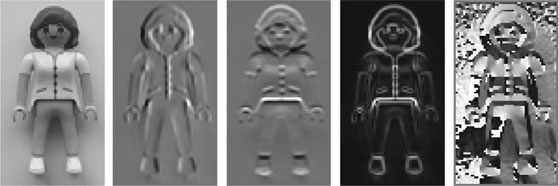
\includegraphics[width=12cm]{images/sobel_kernel_example.png}
	\end{center}	
	\longcaptionsource{Przykład wykrywania krawędzi z wykorzystaniem operatora Sobela}{Od lewej: obraz wejściowy w skali szarości; gradient poziomy (jasny kolor - wartości dodatnie, ciemny kolor - wartości ujemne); gradient pionowy (jasny kolor - wartości dodatnie, ciemny kolor - wartości ujemne); moduł gradientu; orientacja gradientu}{\cite{Treiber2010}}
\label{fig:Sobel_przyklad}
\end{figure}

Innym sposobem usuwania zakłóceń wykonanie wstępnej filtracji dolnoprzepustowej, przy czym stosowany filtr powinien być kołowo-symetryczny \cite{Szeliski2011} (powinien wygładzać obraz w każdym kierunku). Najczęściej wykorzystywany jest filtr Gaussa, posiadający tą właściwość. Ze względu na liniowość operacji różniczkowania i splotu, gradient filtrowanego obrazu można wyliczyć z równania \ref{equ:Gradient_filtrowany} \cite{Szeliski2011}.
\begin{equation}
\label{equ:Gradient_filtrowany}
	\vec{J_{\sigma}}(\vec{x}) =  \nabla (G_{\sigma}(\vec{x}) \ast I (\vec{x})) = (\nabla G_{\sigma})(\vec{x}) \ast I(\vec{x})
\end{equation}

\noindent
gdzie:

\begin{conditions}
	G_{\sigma} & maska filtru Gaussa o wariancji $\sigma$ \\
\end{conditions}

Gradient przefiltrowanego obrazu można więc wyznaczyć poprzez wykonanie jednej operacji konwolucji pomiędzy nim a poziomymi i pionowymi pochodnymi cząstkowymi maski Gaussa \cite{Szeliski2011}.

Częstym wymaganiem stawianym algorytmom wykrywania krawędzi jest ograniczenie zbioru wynikowego do krawędzi izolowanych, tj. zbioru pojedynczych pikseli zlokalizowanych wzdłuż krawędzi \cite{Szeliski2011}. W celu wyodrębniania tych pikseli należy znaleźć w całym zbiorze pikseli krawędzi elementy o maksymalnym module gradientu w kierunku prostopadłym do samej krawędzi \cite{Szeliski2011}. Realizacja tego zadania sprowadza się do wyznaczenia pochodnej kierunkowej obliczonego wcześniej gradientu wzdłuż jego kierunku (zgodnie z równaniem \ref{equ:Laplasjan_filtru_Gaussa}) oraz odnalezienia punktów zmiany jej znaku (ang. \textit{zero crossing}) \cite{Szeliski2011}.
\begin{equation}
\label{equ:Laplasjan_filtru_Gaussa}
	S_\sigma (\vec{x}) = \nabla \vec{J_{\sigma}} (\vec{x}) = \nabla^2 G_\sigma (\vec{x}) \ast I(\vec{x}
\end{equation}

\noindent
gdzie:

\begin{conditions}
	\nabla^2 & laplasjan \\
	S_\sigma (\vec{x}) & wartość funkcji znaku dla współrzędnych $\vec{x}$ \\
\end{conditions}

Maska po wykonaniu splotu $\nabla^2 G_\sigma (\vec{x})$ nazywana jest laplasjanem filtru Gaussa (ang. \textit{Laplacian of Gaussian}, w skrócie \textit{LoG}). Ze względu na złożoność obliczeniową operacja \textit{LoG} jest często aproksymowana przez przytoczoną wcześniej operacją \textit{DoG} \cite{Szeliski2011}. Wykrywanie zmiany znaku odbywa się poprzez porównanie wartości funkcji znaku $S_\sigma$ dla dwóch sąsiednich pikseli. W przypadku jej wystąpienia, na podstawie współrzędnych tych pikseli określane jest położenie punktu należącego do krawędzi (może mieć on charakter sub-pikselowy), oraz, ewentualnie interpolowana jest wartość jego gradientu \cite{Szeliski2011}. Punkt sklasyfikowany jako należący do krawędzi bywa w literaturze określany jako \textit{edgel} \cite{Szeliski2011} (połączenie słów \textit{edge} i \textit{element}).

Przedstawione wyżej metody wykrywania krawędzi operują jedynie na obrazach w skali szarości. Trywialnym sposobem rozszerzenia dziedziny ich działania na obrazy kolorowe jest osobne wykonanie dla każdej składowej koloru. Może to jednak prowadzić do wystąpienia niepożądanych zjawisk, takich jak np. wzajemne znoszenie się gradientów różnych składowych przy ich sumowaniu \cite{Szeliski2011}. Istnieją bardziej zaawansowane algorytmy rozwiązania tego problemu, nie zostaną jednak omówione w niniejszej pracy. 

Kolejnym zagadnieniem związanym z wykrywaniem krawędzi jest łączenie pikseli krawędzi izolowanych w ciągłe \textbf{kontury}, które w zależności od zastosowania, mogą być bardziej użyteczne \cite{Szeliski2011}. Kontur jest listą lub posortowaną tablicą punktów krawędzi \cite{Szeliski2011}, ma więc strukturę uporządkowaną. Jeżeli punkt krawędzi wykryto na podstawie zmiany znaku pewnej funkcji (jak, np. opisano powyżej), operacja łączenia w ciąg sprowadza się do wybrania jednego elementu i dołączaniu jego kolejnych sąsiadów w obu kierunkach \cite{Szeliski2011}.

\subsection{Proste i krzywe matematyczne}
\label{subsec:Proste_i_krzywe_matematyczne}
W wyniku operacja łączenia punktów krawędzi otrzymuje się reprezentację krzywej w przestrzeni 2-D w postaci należących do niej punktów \cite{Szeliski2011}. Na ich podstawie można następnie wykonać aproksymację, mającą na celu uzyskanie reprezentacji w postaci \textbf{prostej lub krzywej opisanej równaniami matematycznymi}. Przy zastosowaniu odpowiednich metod (w szczególności transformaty Hougha) jest to możliwe nawet w przypadku wystąpienia na obrazie przerw lub przysłonięć konturu \cite{Szeliski2011}. Same cechy o tej postaci nie są jednak użyteczne w przypadku zadania śledzenia obiektów, wobec czego zagadnienie to nie zostanie szerzej omówione.

\section{Analiza ruchu}
\label{sec:Analiza_ruchu}

\subsection{Ruch w sekwencji obrazów}
\label{subsec:Ruch_w_sekwencji_obrazow}
Analiza ruchu obserwowanego w sekwencji obrazów jest kwintesencją algorytmów śledzenia obiektów, oraz wielu innych, jak np. kompresja video (w tym \textit{MPEG} i \textit{H.263}), stabilizacja obrazu, obrazowa diagnostyka medyczna, rekonstrukcja sceny 3-D na podstawie obrazu z poruszającej się kamery, etc. \cite{Szeliski2011}. Ze względu na postać przetwarzanych danych - sekwencje zamiast pojedynczych obrazów - analiza ruchu jest stosunkowo wymagająca obliczeniowo oraz pamięciowo. 

\begin{figure}[!htb]
	\begin{center}
		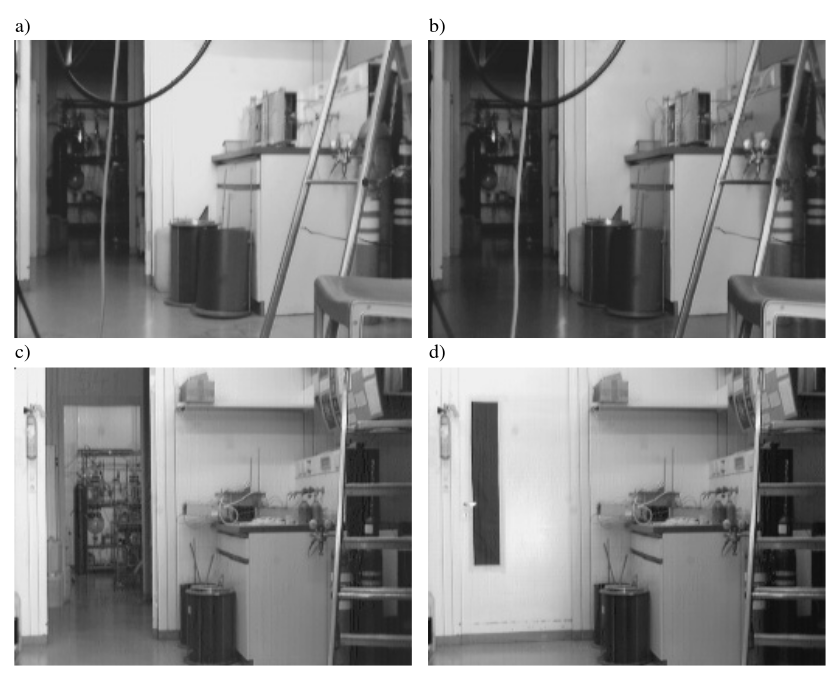
\includegraphics[width=12cm]{images/motion_illumination_change_example.png}
	\end{center}	
	\longcaptionsource{Przykład różnic pomiędzy kolejnymi obrazami sekwencji}{Definicja par: a) poprzedza b); c) poprzedza d)}{\cite{Jaehne2005}}
\label{fig:Zmiany_w_sekwencji_przyklad}
\end{figure}

Intuicyjnie, opiera się ona na obserwowaniu różnic pomiędzy dwoma kolejnymi klatkami \cite{Jaehne2005}. W trywialnym ujęciu, można ją zrealizować właśnie poprzez odjęcie od siebie dwóch kolejnych klatek, czyli poprzez wyznaczenie różnicy wartości pikseli o tych samych współrzędnych. Takie podejście okazuje się jednak bardzo szybko prowadzić do błędnej interpretacji, ponieważ zmiany wartości pikseli wynikają nie tylko z ruchu obiektów, ale również z występujących zmian iluminacji \cite{Jaehne2005}. Mogą mieć one charakter globalny - zmienia się oświetlenie całej sceny, lub lokalny - przemieszczenie lub inna zmiana stanu obiektu na scenie zmienia sposób w jaki odbija on światło, tym samym zmieniając iluminację innych obiektów w jego otoczeniu. Przykładowo, na rysunku \ref{fig:Zmiany_w_sekwencji_przyklad} przedstawiono dwie pary obrazów tej samej sceny a na rysunku \ref{fig:Roznica_obrazow_przyklad} różnice pomiędzy obrazami tych par. W pierwszej z nich zmianie ulega oświetlenie całej sceny, zmianie ulega iluminacja całej sceny, nie występuje natomiast ruch obiektów, co objawia się ogólną, niewielką zmianą wartości pikseli. W drugiej zamknięcie drzwi, a więc ich ruch, skutkuje dużą zmianą wartości pikseli przynależących do ich obszaru oraz niewielkimi lokalnymi zmianami widocznymi na innych obiektach.

\begin{figure}[!htb]
	\begin{center}
		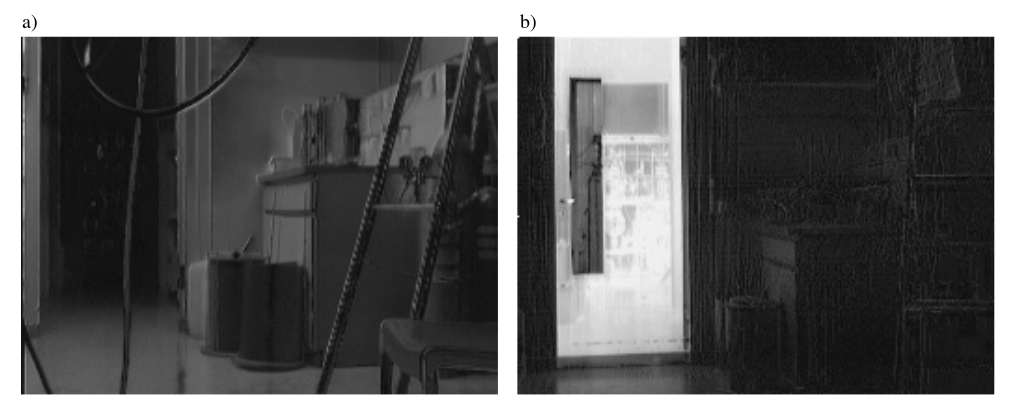
\includegraphics[width=12cm]{images/image_difference_example.png}
	\end{center}	
	\longcaptionsource{Przykład wyniku operacji odejmowania dwóch kolejnych obrazów sekwencji}{Objaśnienie: a) odejmowanie obrazów z rysunku \ref{fig:Zmiany_w_sekwencji_przyklad} a) i b); b) odejmowanie obrazów z rysunku \ref{fig:Zmiany_w_sekwencji_przyklad} c) i d)}{\cite{Jaehne2005}}
\label{fig:Roznica_obrazow_przyklad}
\end{figure}

Ruch w sekwencji obrazów ujawnia się więc poprzez zmiany wartości pikseli o charakterze przestrzennym i czasowym \cite{Jaehne2005}. W celu jego analizy konieczna jest wiedza o związku pomiędzy punktami na obrazie pierwotnym i następującym, tzn. zdefiniowanie wektorów przemieszczeń, co nie zawsze jest to możliwe w sposób jednoznaczny. Przykładowo, na obrazie obserwowany jest pewien region $x_i$ (rysunek \ref{fig:Problem_apertury}). W zależności od sposobu jego zdefiniowania, ścisłe określenie korespondencji pomiędzy tym regionem a odpowiadającym mu regionem na następnym obrazie sekwencji może być możliwe (rysunek \ref{fig:Problem_apertury}a) lub nie (rysunek \ref{fig:Problem_apertury}b i c). Zjawisko to nosi nazwę \textbf{problemu apertury}.

\begin{figure}[!htb]
	\begin{center}
		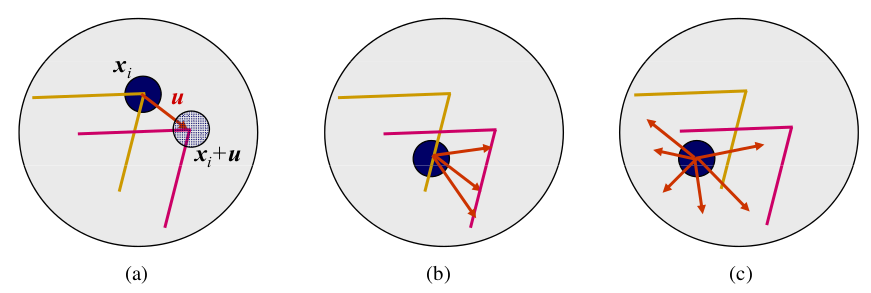
\includegraphics[width=12cm]{images/aperture_problem.png}
	\end{center}	
	\longcaptionsource{Warunki wystąpienia problemu apertury}{Krawędź obiektu zainteresowania na obrazie pierwotnym oznaczono kolorem żółtym, na obrazie następującym kolorem fioletowym. Zdefiniowano pewien region opisywany przez współrzędne jego środka $x_i$, poszukiwany jest wektor przemieszczenia $u$, pozwalający na wyznaczenie jego kolejnych współrzędnych. Możliwe przypadki: a) wektor $u$ może zostać wyznaczony w sposób jednoznaczny; b) ze względu na informacje zawarte w wybranym regionie $x_i$ na obrazie następującym można wyznaczyć wiele dopasowanych do niego regionów $x_i + u$, tzn. wektor $u$ może przyjąć wiele różnych postaci; c) informacje zawarte w regionie $x_i$ nie narzucają żadnych więzów dotyczących jego kolejnego położenia}{\cite{Szeliski2011}}
\label{fig:Problem_apertury}
\end{figure}

Problem apertury jest szczególnym przypadkiem \textbf{problemu korespondencji}, polegające na niemożliwości określenia korespondencji punktów na dwóch kolejnych obrazach w sekwencji \cite{Jaehne2005}. Jego naturę dobrze przedstawia przykład z rysunku \ref{fig:Problem_korespondencji}, na którym przedstawiono zbiór poruszających się, identycznych cząsteczek. Utworzenie powiązań pomiędzy ich pierwotnymi a wtórnymi wystąpieniami jest wykonalne, o ile odległości pomiędzy nimi są znacząco większe od długości wektorów przesunięć (rysunek \ref{fig:Problem_korespondencji}a), w przeciwnym wypadku jest niemożliwe (rysunek \ref{fig:Problem_korespondencji} b)). Zjawisko to można ograniczyć zwiększając częstotliwość próbkowania obrazów, co przekłada się na zmniejszenie modułów wektorów przesunięć \cite{Jaehne2005}. Jego całkowita eliminacja nie jest jednak możliwa przy braku założenia minimalnej dopuszczalnej odległości między cząsteczkami.

\begin{figure}[!htb]
	\begin{center}
		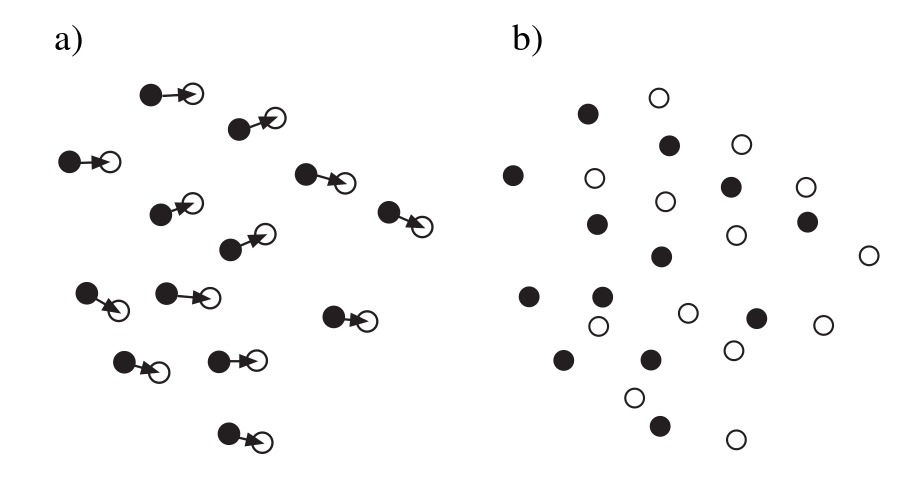
\includegraphics[width=12cm]{images/correspondence_problem.png}
	\end{center}	
	\longcaptionsource{Przykład występowania problemu korespondencji}{Czarne koła obrazują pierwotne a białe wtórne położenia nierozróżnialnych cząsteczek. Występowanie problemu korespondencji: a) względne przesunięcia cząsteczek są małe w porównaniu do odległości między nimi, dopasowanie polega na odnalezieniu najbliższej cząsteczki; b) duże wartości modułów wektorów przesunięć uniemożliwiają wykonanie dopasowania}{\cite{Jaehne2005}}
\label{fig:Problem_korespondencji}
\end{figure}

Przedstawione powyżej przykłady obrazują podstawowy problem analizy ruchu, tzn. brak identyczności pomiędzy fizyczną korespondencją rzeczywistych obiektów a wizualną korespondencją występującą na obrazie \cite{Jaehne2005}. Określenie wizualnej korespondencji pomiędzy obiektami na dwóch obrazach jest możliwe, nawet jeżeli nie występuje pomiędzy nimi fizyczna korespondencja, natomiast fizyczna korespondencja dwóch obiektów nie musi skutkować ich wizualną korespondencją na obrazie \cite{Jaehne2005}.

\subsection{Przepływ optyczny}
\label{subsec:Przeplyw_optyczny}
W celu uchwycenia zależności pomiędzy ruchem występującym w sekwencji obrazów a zmianami wartości pikseli konieczne jest wprowadzenie dwóch pojęć - \textbf{pola ruchu} (ang. \textit{motion field}) oraz \textbf{przepływu optycznego} (ang. \textit{optical flow}) \cite{Jaehne2005}. Pole ruchu $\vec{u} = [u_1, u_2]^T = [u, v]^T$ to pole wektorów rzeczywistego ruchu obiektów w przestrzeni trójwymiarowej rzutowanych na dwuwymiarową płaszczyznę obrazu, określone dla każdego jego piksela, o wymiarze prędkości \cite{Jaehne2005} \cite{Baker2011}. Przepływ optyczny $\vec{f} = [f_1, f_2]^T$ jest estymacją pola ruchu \cite{Szeliski2011}, wyznaczaną na podstawie obserwowanych przemieszczeń (,,przepływu'') poszczególnych pikseli obrazu rozróżnianych poprzez ich wartość \cite{Jaehne2005} \cite{Baker2011} \cite{Horn1981}. Pole ruchu i przepływ optyczny są identyczne tylko jeśli obiekty poruszające się na scenie nie zmieniają irradiancji płaszczyzny obrazu \cite{Jaehne2005}. Przykładową sekwencję obrazów oraz wyznaczony dla niej przepływ optyczny przedstawiono na rysunku \ref{fig:Przeplyw_optyczny}.

\begin{figure}[!htb]
	\begin{center}
		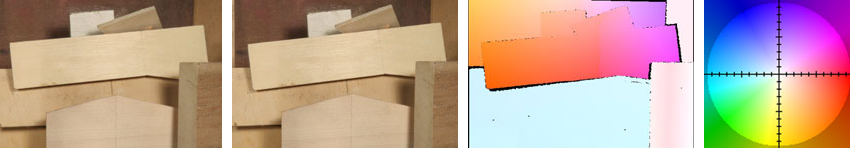
\includegraphics[width=16cm]{images/optical_flow_example.png}
	\end{center}	
	\longcaptionsource{Przykład wizualizacji przepływu optycznego}{Od lewej: dwa kolejne obrazy sekwencji, wizualizacja wyznaczonego przepływu optycznego, kodowanie modułu przepływu (jednostki na osiach mają wymiar pikseli). Pomiędzy klatkami nastąpił ruch sztywnego obiektu na pierwszym planie, tło pozostało nieruchome (brak ruchu kamery)}{\cite{Baker2011}}
\label{fig:Przeplyw_optyczny}
\end{figure}

Przepływ optyczny obliczany jest dla każdego piksela obrazu. Większość metod jego wyznaczania opiera się o optymalizację pewnej funkcji globalnej energii $E_G$ o postaci \cite{Baker2011}:
\begin{equation}
\label{equ:Energia_globalna}
	E_G = E_D + \lambda E_P
\end{equation}

\noindent
gdzie:

\begin{conditions}
	E_D & term danych - określenie stopnia spójności przepływu optycznego \\
	E_P & term nadrzędny - dookreślający problem poprzez preferowanie przepływów o określonym charakterze (np. płynnych) \\
	\lambda & współczynnik wagowy \\
\end{conditions}

Podstawowa definicja termu danych opiera się o założenie \textbf{warunku stałej jasności} (ang. \textit{brightness constancy}), tzn. że piksel odpowiadający pojedynczemu punktowi poruszającego się obiektu zmieniając położenie na obrazie nie zmienia swojej wartości lub koloru \cite{Baker2011}. Formalną postać tego warunku przedstawia równanie \ref{equ:Warunek_stalej_jasnosci}. 
\begin{equation}
\label{equ:Warunek_stalej_jasnosci}
	I(x, y, t) = I(x + u, y + v, t + 1)
\end{equation}

\noindent
gdzie:

\begin{conditions}
	I(x, y, t) & wartość piksela $(x, y)$ na obrazie $I$ w chwili $t$ \\
	(u(x, y, t), v(x, y, t)) & przepływ \\
\end{conditions}

Rozwinięcie równania \ref{equ:Warunek_stalej_jasnosci} w szereg Taylora pierwszego rzędu pozwala na wyznaczenie \textbf{równania przepływu optycznego} (ang. \textit{optical flow constraint}):
\begin{equation}
\label{equ:Rownanie_przeplywu_optycznego}
	u \frac{\partial I}{\partial x} + v \frac{\partial I}{\partial y} + \frac{\partial I}{\partial t} = 0
\end{equation}

Równania \ref{equ:Warunek_stalej_jasnosci} i \ref{equ:Rownanie_przeplywu_optycznego} zawierają po dwie niewiadome, elementy nieznanego przepływu $u(x, y, t), v(x, y, t)$, przy jednoczesnym narzuceniu pojedynczego ograniczenia. Oznacza to, że zagadnienie wyznaczenia przepływu jest niedookreślone, stąd konieczność wprowadzenia do równania \ref{equ:Energia_globalna} termu nadrzędnego. Jest to również formalna przyczyna występowania wspomnianego wcześniej problemu apertury \cite{Baker2011}. Oba równania mogą służyć do wyznaczenia postaci termu danych, przy czym ich znaczenie jest praktycznie tożsame, alternatywę stanowi założenie o wysokim współczynniku korelacji pomiędzy dwoma kolejnymi obrazami \cite{Baker2011}. Stosowane równanie jest przekształcane do postaci, z której wylicza się wartość błędu dla każdego piksela. Wartości błędów są następnie agregowane, w wyniku czego otrzymuje się funkcję kary, jak np. w algorytmie Horna-Schuncka \cite{Horn1981} \cite{Baker2011} \cite{Karasulu2013}:
\begin{equation}
\label{equ:Funkcja_kary}
	E_D = \sum\limits_{x,y} (u \frac{\partial I}{\partial x} + v \frac{\partial I}{\partial y} + \frac{\partial I}{\partial t})^2
\end{equation}

W celu zwiększenia odporności na zmiany wyglądu sceny nie wynikające z ruchu, niektóre metody zamiast wartości pikseli używają cech, np. opisanych w podrozdziale \ref{sec:Ekstrakcja_i_deskrypcja_cech_obrazu} punktów charakterystycznych \textit{SIFT} \cite{Baker2011}, lub innych, specjalnie do tego przystosowanych. 
Zwiększenie odporności można również uzyskać poprzez wprowadzenie do równania \ref{equ:Warunek_stalej_jasnosci} zmiany wartości piksela wprost \cite{Baker2011}

\begin{equation}
\label{equ:Warunek_stalej_jasnosci_zmodyfikowany}
	g(x,y) I(x, y, t) = I(x + u, y + v, t + 1) + b(x, y)
\end{equation}

\noindent
gdzie:

\begin{conditions}
	g(x,y) & współczynnik skalujący \\
	b(x,y) & współczynnik przesunięcia \\
\end{conditions}

Oczywistą konsekwencją takiego działania jest zwiększenie liczby niewiadomych do czterech, wymaga więc ono narzucenia na zmiany zmianę wartości piksela zdefiniowaną przez $g(x,y)$ i $b(x,y)$ odpowiednich więzów \cite{Baker2011}.

Term nadrzędny w równaniu \ref{equ:Energia_globalna} ma za zadanie wprowadzenie dodatkowych ograniczeń, umożliwiających wyznaczenie jego jednoznacznego rozwiązania. Najczęściej dotyczą one gładkości przepływu \cite{Baker2011}. W najprostszej postaci, stosowanej w algorytmie Horna-Schuncka, preferowany jest przepływ o małym gradiencie, sam term nadrzędny przyjmuje postać \cite{Horn1981} \cite{Baker2011}:

\begin{equation}
\label{equ:Term_nadrzedny}
	E_P = \sum\limits_{x,y}[(\frac{\partial u}{\partial x})^2 +(\frac{\partial u}{\partial y})^2 + (\frac{\partial v}{\partial x})^2 + (\frac{\partial v}{\partial y})^2] 
\end{equation}

Ulepszenie tej koncepcji polega na nadaniu składnikom sumy wag, wyznaczanych na podstawie pewnej funkcji zmieniającej wartość w zależności od przestrzennego położenia rozpatrywanego piksela. W szczególności, może ona operować na gradiencie obrazu (zmodyfikowaną postać termu nadrzędnego przedstawia równanie \ref{equ:Term_nadrzedny_wazony}) i maleć wraz z jego wzrostem, co zmniejsza znaczenie pikseli należących do krawędzi. Jest to korzystne, ponieważ zaburzenie ciągłości przepływu jest bardziej prawdopodobne właśnie na krawędziach \cite{Baker2011}. 

\begin{equation}
\label{equ:Term_nadrzedny_wazony}
	E_P = \sum\limits_{x,y} w(\nabla I) [(\frac{\partial u}{\partial x})^2 +(\frac{\partial u}{\partial y})^2 + (\frac{\partial v}{\partial x})^2 + (\frac{\partial v}{\partial y})^2] 
\end{equation}

\noindent
gdzie:

\begin{conditions}
	w(\nabla I) & funkcja wagi \\
\end{conditions}

Innym możliwym założeniem służącym do wyznaczenia termu nadrzędnego jest założenie sztywności, np. preferujący przepływ przebiegający wzdłuż linii epipolarnych \cite{Baker2011}. 

Oba składniki równania energii globalnej (równanie \ref{equ:Energia_globalna}) mają charakter funkcji kary. Wyznaczenie przepływu dla danego piksela polega na rozwiązaniu zadania jej minimalizacji, w którym zmiennymi decyzyjnymi są elementy definiującego go wektora $(u, v)$. Dwie podstawowe metody stosowane w tym celu to \textbf{metoda gradientu prostego} oraz \textbf{rachunek wariacyjny} \cite{Baker2011}. 

Metoda gradientu prostego polega na iteracyjnym przybliżaniu rozwiązania optymalnego kolejnymi punktami w przestrzeni poszukiwań wyznaczanymi na podstawie gradientu funkcji celu, w tym przypadku:

\begin{equation}
\label{equ:Metoda_gradientu_prostego}
	-\nabla E_G(\vec{f}) = - \frac{\partial E_G}{\partial \vec{f}}
\end{equation}

\noindent
gdzie:

\begin{conditions}
	 \vec{f} & wektor przepływu $\vec{f} = (u, v)$ \\
\end{conditions}

W przypadku zastosowania rachunku wariacyjnego zakłada się, że energię globalną $E_G$ można przedstawić w formie \cite{Baker2011}:

\begin{equation}
\label{equ:Rachunek_wariacyjny}
	E_G = \iint E(u(x,y), v(x,y), x, y, u_x, u_y, v_x, v_y) \,dx \,dy
\end{equation}

\noindent
gdzie:

\begin{conditionseq}
	 u_x & $\frac{\partial u}{\partial x}$ \\
	 u_y & $\frac{\partial u}{\partial y}$ \\
	 v_x & $\frac{\partial v}{\partial x}$ \\
	 v_y & $\frac{\partial v}{\partial y}$ \\
\end{conditionseq}

Składowe przepływu $u$ i $v$ są w tym przypadku traktowane jako funkcje położenia $u(x,y)$ i $v(x,y)$, ich parametryzacja następuje później. Minimum funkcjonału energii $E_G$ jest wyznaczane na podstawie równań Eulera-Lagrange'a \cite{Horn1981} \cite{Baker2011}:

\begin{equation}
\label{equ:Rownania_Eulera_Lagrangea_u}
	\frac{\partial E_G}{\partial u} - \frac{\partial}{\partial x} \frac{\partial E_G}{\partial u_x} - \frac{\partial}{\partial y} \frac{\partial E_G}{\partial u_y} = 0
\end{equation}

\begin{equation}
\label{equ:Rownania_Eulera_Lagrangea_v}
	\frac{\partial E_G}{\partial v} - \frac{\partial}{\partial x} \frac{\partial E_G}{\partial v_x} - \frac{\partial}{\partial y} \frac{\partial E_G}{\partial v_y} = 0
\end{equation}

Przykładowo, dla algorytmu Horna-Schuncka $E_G$ przyjmuje postać \cite{Horn1981}:
\begin{equation}
\label{equ:Energia_globalna_Horn_Schunck}
		E_G = \iint (I_x u + I_y v + I_t)^2 + \alpha^2 (u_x^2 + u_y^2 + v_x^2 + v_y^2) \,dx \,dy
\end{equation}

\noindent
gdzie:

\begin{conditionseq}
	 I_x & $\frac{\partial I}{\partial x}$ \\
	 I_y & $\frac{\partial I}{\partial y}$ \\
	 I_t & $\frac{\partial I}{\partial t}$ \\
\end{conditionseq}

\begin{conditions}
	 \alpha^2 & współczynnik wagi \\
\end{conditions}

Po podstawieniu równania \ref{equ:Energia_globalna_Horn_Schunck} do równań \ref{equ:Rownania_Eulera_Lagrangea_u} i \ref{equ:Rownania_Eulera_Lagrangea_v}:

\begin{equation}
\label{equ:Euler_Lagrange_Horn_Schunck_u}
	I_x^2 u + I_x I_y v = \alpha^2 \nabla^2 u - I_x I_t
\end{equation}

\begin{equation}
\label{equ:Euler_Lagrange_Horn_Schunck_v}
	I_x I_y u + I_y^2 v = \alpha^2 \nabla^2 v - I_y I_t
\end{equation}

\noindent
gdzie:

\begin{conditions}
	 \nabla^2 & laplasjan \\
\end{conditions}

Laplasjany $\nabla^2 u$ i $\nabla^2 v$ w równaniach \ref{equ:Euler_Lagrange_Horn_Schunck_u} i \ref{equ:Euler_Lagrange_Horn_Schunck_v} są aproksymowane przez różnicę wartości rozpatrywanego piksela $u(x,y)$ lub $v(x,y)$ oraz średniej ważonej wartości pikseli jego otoczenia $\bar{u}(x,y)$ lub $\bar{v}(x,y)$ \cite{Horn1981}:
\begin{equation}
\label{equ:Aproksymacja_laplasjanu}
	\nabla^2 u  \approx \bar{u}(x,y) - u(x,y)
	\, \, \, \, \, \,
	\nabla^2 v  \approx \bar{v}(x,y) - v(x,y)
\end{equation}

Po podstawieniu równania \ref{equ:Aproksymacja_laplasjanu} do równań \ref{equ:Euler_Lagrange_Horn_Schunck_u} i \ref{equ:Euler_Lagrange_Horn_Schunck_v} i wykonaniu przekształceń, otrzymuje się układ dwóch równań z dwiema niewiadomymi $(u,v)$:

\begin{equation}
\label{equ:Horn_Schunck_u}
	(\alpha^2 + I_x^2 + I_y^2)(u - \bar{u}) = -I_x(I_x \bar{u} + I_y \bar{v} + I_t)
\end{equation}

\begin{equation}
\label{equ:Horn_Schunck_v}
	(\alpha^2 + I_x^2 + I_y^2)(v - \bar{v}) = -I_v(I_x \bar{u} + I_y \bar{v} + I_t)
\end{equation}

Wyznaczenie przepływu optycznego polega na rozwiązaniu układu równań \ref{equ:Horn_Schunck_u} i \ref{equ:Horn_Schunck_v} dla każdego piksela obrazu. Ze względu na dużą złożoność obliczeniową takiego podejścia, lepszym rozwiązaniem jest iteracyjne wyliczanie kolejnych wartości $(u_{n+1}, v_{n+1})$ na podstawie estymowanych wartości pochodnych $I_x$, $I_y$ i $I_t$ oraz średniej z poprzednich wartości $(u_n, v_n)$, przy założeniu zerowych warunków początkowych:

\begin{equation}
\label{equ:Horn_Schunck_iteracyjnie_u}
	u_{n+1} = \bar{u}_n - I_x \frac{I_x \bar{u}_n + I_y \bar{v}_n + I_t}{\alpha^2 + I_x^2 + I_y^2}
\end{equation}

\begin{equation}
\label{equ:Horn_Schunck_iteracyjnie_v}
	v_{n+1} = \bar{v}_n - I_y \frac{I_x \bar{u}_n + I_y \bar{v}_n + I_t}{\alpha^2 + I_x^2 + I_y^2}
\end{equation}

Powyższe rozważania dotyczą metod wyznaczania przepływu optycznego dla każdego piksela obrazu, który z tego powodu określa się mianem \textbf{gęstego} (ang. \textit{dense}). Alternatywnym podejściem, realizowanym np. przez algorytm Lucasa-Kanade-Tomasi \ref{sec:Algorytm_Lucasa_Kanade}, jest wyznaczenie przepływu optycznego w postaci \textbf{rzadkiej} (ang. \textit{sparse}), tzn. jedynie dla wybranego zbioru punktów obrazów, np. wykrytych punktów charakterystycznych \cite{Karasulu2013}. Gęsty przepływ optyczny jest z natury dokładniejszą estymacją pola ruchu, jednak jego wyznaczanie jest znacznie bardziej złożone obliczeniowo. 